% This file was created with tikzplotlib v0.10.1.
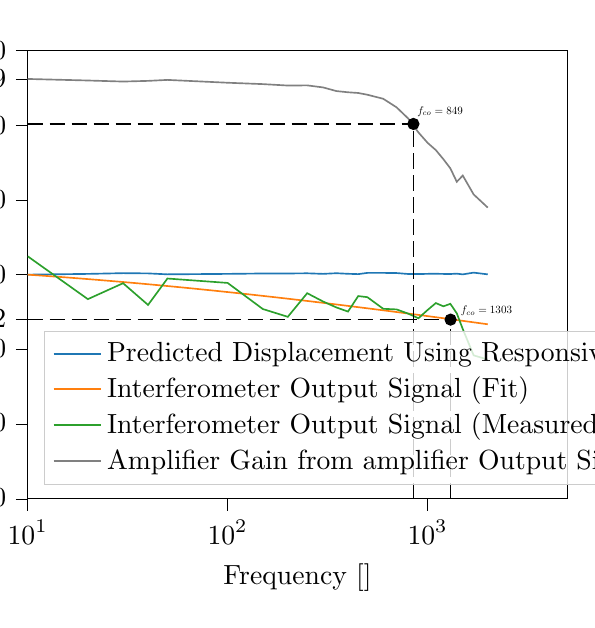
\begin{tikzpicture}[
trim axis left,
trim axis right
]

\definecolor{darkgray176}{RGB}{176,176,176}
\definecolor{darkorange25512714}{RGB}{255,127,14}
\definecolor{forestgreen4416044}{RGB}{44,160,44}
\definecolor{gray}{RGB}{128,128,128}
\definecolor{lightgray204}{RGB}{204,204,204}
\definecolor{steelblue31119180}{RGB}{31,119,180}

\begin{axis}[
legend cell align={left},
legend style={
  fill opacity=0.8,
  draw opacity=1,
  text opacity=1,
  at={(0.03,0.03)},
  anchor=south west,
  draw=lightgray204
},
log basis x={10},
tick align=outside,
tick pos=left,
x grid style={darkgray176},
xlabel={Frequency [\si{\hertz}]},
xmin=10, xmax=5000,
xmode=log,
xtick style={color=black},
xtick={1,10,100,1000,10000,100000},
xticklabels={
  \(\displaystyle {10^{0}}\),
  \(\displaystyle {10^{1}}\),
  \(\displaystyle {10^{2}}\),
  \(\displaystyle {10^{3}}\),
  \(\displaystyle {10^{4}}\),
  \(\displaystyle {10^{5}}\)
},
y grid style={darkgray176},
ylabel={Piezo Displacement [\si{\decibel\meter}] 
 Amplifier Gain [\si{\decibel}]},
ymin=-30, ymax=30,
ytick style={color=black},
ytick={-30,-20,-10,0,10,20,30,-6.02059991327962,26.1908498701312},
yticklabels={
  \ensuremath{-}30.00,
  \ensuremath{-}20.00,
  \ensuremath{-}10.00,
  0.00,
  10.00,
  20.00,
  30.00,
  \ensuremath{-}6.02,
  26.19
}
]
\addplot [draw=black, fill=black, forget plot, mark=*, only marks]
table{%
x  y
1303.43139633966 -6.02059991327962
849.466702481979 20.1702499568515
};
\addplot [semithick, steelblue31119180]
table {%
10 0
20 0.100617896105146
30 0.198893625380764
40 0.165745580404855
50 0.041189907796974
100 0.102616289997218
150 0.154728844119903
200 0.154795052292623
250 0.180305658375857
300 0.105429917926561
350 0.191051124205303
400 0.113549382361036
450 0.0699768421296668
500 0.23409779278967
600 0.234753849232389
700 0.212913443872192
800 0.088342707735542
900 0.0764594022052211
1000 0.108225997226808
1100 0.118703312984083
1200 0.0968363473802095
1300 0.0849312534255893
1400 0.134735812663185
1500 0.0346139292688428
1700 0.269274644398441
2000 0.0385064340527114
};
\addlegendentry{Predicted Displacement Using Responsivity}
\addplot [semithick, darkorange25512714]
table {%
10 0
10.5497635804178 -0.0426741405953974
11.1297511602709 -0.0858942623412657
11.7416243449738 -0.129661840454712
12.3871360889551 -0.173978215770973
13.0681357176937 -0.218844593397971
13.7865742258481 -0.264262041502821
14.5445098666579 -0.310231490232896
15.3441140486294 -0.356753730773719
16.1876775564007 -0.403829414545732
17.0776171136062 -0.451459052541666
18.0164823065441 -0.499643014805914
19.006962888482 -0.548381530057091
20.0518964855259 -0.597674685454527
21.1542767261308 -0.647522426509256
22.3172618175414 -0.697924557139673
23.5441835937345 -0.748880739871724
24.838557060785 -0.800390496183232
26.2040904669998 -0.852453206991561
27.6446959266726 -0.905068113283622
29.1645006278934 -0.958234316886816
30.767858656522 -1.01195078137927
32.4593634702017 -1.06621633313739
34.2438610581476 -1.12102966251859
36.1264638244131 -1.17638932517647
38.1125652344073 -1.23229374350591
40.2078552666246 -1.28874120821481
42.4183367138545 -1.34572988001933
44.7503423805719 -1.40325779145901
47.2105532257782 -1.46132284882806
49.8060175032689 -1.51992283421882
52.5441709541636 -1.57905540767323
55.4328581095479 -1.63871810943801
58.4803547642573 -1.69890836231894
61.6953916861872 -1.75962347412965
65.0871796290546 -1.8208606402301
68.6654357202708 -1.88261694614973
72.4404112995229 -1.94488937029044
76.4229212878189 -2.00767478670407
80.6243751711364 -2.07096996793926
85.0568096874393 -2.13477158795247
89.732923310707 -2.19907622507786
94.6661126307717 -2.26388036505057
99.870510733184 -2.32918040407828
105.361027689066 -2.39497265195548
111.15339327095 -2.46125333521537
117.264202016972 -2.52801860031386
123.71096077254 -2.59526451684066
130.512138845663 -2.6629870807521
137.68722091964 -2.73118221762071
145.256762874695 -2.79984578589636
153.242450678484 -2.86897358017429
161.667162514183 -2.93856133446493
170.555034324161 -3.00860472546094
179.931528956993 -3.07909937579696
189.823509115937 -3.15004085729736
200.259314317841 -3.22142469420801
211.268842082979 -3.29324636640762
222.883633588404 -3.36550131259482
235.136964030212 -3.43818493344706
248.063937953593 -3.51129259474764
261.701589823782 -3.58481963047736
276.088990126036 -3.65876134586752
291.267357298597 -3.73311302041097
307.280175819327 -3.80786991082831
324.17332078431 -3.88302725398644
341.995189335339 -3.95858026976672
360.796839312804 -4.03452416388043
380.632135531205 -4.11085413062911
401.557904096374 -4.18756535560785
423.634095206482 -4.26465301834938
446.923954903256 -4.34211229490747
471.494206265464 -4.41993836037788
497.415240563737 -4.49812639135548
524.761318924405 -4.57667156832643
553.610785080067 -4.65556907799411
584.046289816417 -4.73481411553814
616.155027758334 -4.81440188680551
650.028987173616 -4.8943276104333
685.765213510006 -4.97458651990254
723.466087420527 -5.05517386552278
763.239618073639 -5.13608491634723
805.199752588523 -5.21731496201846
849.466702481979 -5.29885931454455
896.167288062195 -5.38071331000599
945.435301756029 -5.46287231019359
997.411891410702 -5.54533170417772
1052.24596466802 -5.62808690980944
1110.09461556962 -5.71113337515409
1171.12357461543 -5.79446657985795
1235.50768356465 -5.87808203644882
1303.43139633966 -5.96197529157127
1375.08930746772 -6.04614192715749
1450.68670957448 -6.13057756153477
1530.4401815265 -6.21527785047054
1614.57820890761 -6.30023848815618
1703.34183860697 -6.38545520813058
1796.98536939376 -6.47092378414485
1895.77708045738 -6.55664003096923
2000 -6.64259980514353
};
\addlegendentry{Interferometer Output Signal (Fit)}
\addplot [semithick, forestgreen4416044]
table {%
10 2.45626167181096
20 -3.27961206470276
30 -1.14768620381086
40 -4.0527120439998
50 -0.519929068192114
100 -1.10851733479257
150 -4.60143214284313
200 -5.64471400944723
250 -2.48440080370199
300 -3.59173346535549
350 -4.39063527614884
400 -4.9440228396236
450 -2.8666310248649
500 -3.01438509433959
600 -4.57087766694543
700 -4.65396205603846
800 -5.21632613156837
900 -5.8407274547744
1000 -4.73040548910604
1100 -3.80457362570566
1200 -4.23941894619464
1300 -3.90503677546332
1400 -5.17397606978555
1500 -7.28112954052816
1700 -10.7995360076244
2000 -11.3679453269758
};
\addlegendentry{Interferometer Output Signal (Measured)}
\path [draw=black, semithick, dash pattern=on 5.55pt off 2.4pt]
(axis cs:1303.43139633966,-30)
--(axis cs:1303.43139633966,-6.02059991327962);

\path [draw=black, semithick, dash pattern=on 5.55pt off 2.4pt]
(axis cs:10,-6.02059991327962)
--(axis cs:1303.43139633966,-6.02059991327962);

\path [draw=black, semithick, dash pattern=on 5.55pt off 2.4pt]
(axis cs:849.466702481979,-30)
--(axis cs:849.466702481979,20.1702499568515);

\path [draw=black, semithick, dash pattern=on 5.55pt off 2.4pt]
(axis cs:10,20.1702499568515)
--(axis cs:849.466702481979,20.1702499568515);

\addplot [semithick, gray]
table {%
10 26.1908498701312
20 25.9841309579933
30 25.8424755512605
40 25.9339587572483
50 26.0641230070407
100 25.6840837550704
150 25.5001311079422
200 25.3092977104383
250 25.3310054454202
300 25.0594929726463
350 24.568300415676
400 24.4084871217865
450 24.3129023680881
500 24.0782007647374
600 23.5379239870916
700 22.3909042249216
800 20.8984012540715
900 19.0350448406496
1000 17.6442198410529
1100 16.6681174488149
1200 15.4482594017803
1300 14.2274797913939
1400 12.4258711514334
1500 13.260057012421
1700 10.7358594914377
2000 8.9743906742906
};
\addlegendentry{Amplifier Gain from amplifier Output Signal (Measured)}
\draw (axis cs:1403.43139633966,-6.02059991327962) node[
  scale=0.4,
  anchor=south west,
  text=black,
  rotate=0.0
]{$f_{co}= \qty{1303}{\hertz}$};
\draw (axis cs:849.466702481979,20.6702499568515) node[
  scale=0.4,
  anchor=south west,
  text=black,
  rotate=0.0
]{$f_{co}= \qty{849}{\hertz}$};
\end{axis}

\end{tikzpicture}
